\subsection{ECPT on EMT-Linux}
\label{emt:sec:ecpt_impl}

\subsubsection{Emulator-based Toolchain}
\label{emt:sec:eval:emulator}

\noindent
It is challenging to develop OSes for new translation architectures
	without manufactured MMU hardware.
% Despite extensive research on memory architectures, we
We did not find an available toolchain for developing
	and evaluating OS kernels with experimental architectures like ECPT.
% The common practice is to use a performance model 
%	to estimate OS overheads~\cite{self:dmt,margaritov2019asap,yaniv2016hash},
%	or uses full-system simulation on vanilla Linux~\cite{skarlatos2020ecpt}.
The original evaluation of ECPT~\cite{skarlatos2020ecpt}
	collects memory traces from simulation using Simics~\cite{plat:simics}
	on {\it vanilla Linux} 
	and replays traces in SST~\cite{plat:sst} that simulated an ECPT MMU.
Simics is closed-source and only supports existing ISAs.
%	hence, it cannot directly support EMT-Linux with ECPT.

\begin{figure}[H]
	\centering
	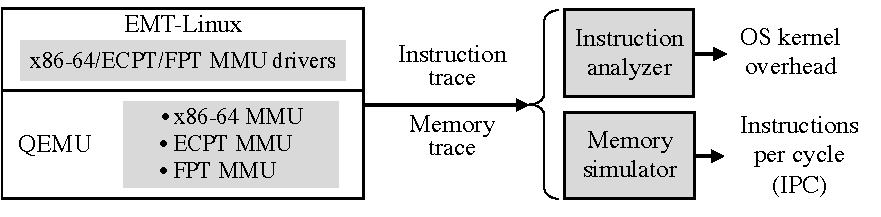
\includegraphics[width=0.65\textwidth]{figs/emu.pdf}
	\caption{\bf Emulator toolchain for OS development and evaluation 
		on experimental memory architectures.}
%	\vspace{-2.5pt}
	\label{emt:fig:eval:emulator}
\end{figure}

We develop an emulator-based toolchain using QEMU~\cite{plat:qemu} (Figure~\ref{emt:fig:eval:emulator}).
% \schai{QEMU's software MMU module ~\cite{} handles all virtual to physical translation requests
%	for every off-TLB memory access in guest OS and applications.
%	We developed our own software MMU with ECPT-based translation logic, as well as Cuckoo Walk Cache (CWC).
%}
% git diff --stat bb4aa8f59e18412cff0d69f14aee7abba153161a -- target
We use QEMU's software MMU mechanism~\cite{plat:qemu:softmmu} to develop an emulated ECPT MMU where 
	we implement ECPT translation logic and hardware caches
	in 3.1K lines of C code.
% The software ECPT MMU 
% \schai{QEMU's software MMU handles all virtual to physical translation requests
% 	for every off-TLB memory access in guest OS and applications to garantee functional correctness.
% }
	% \TODO{intercepts all the MMU instructions @Siyuan please describe
	% some details; and describe how to do instruction analysis in the figure.}
% We implemented the ECPT MMU and ECPT MMU driver together (\S\ref{emt:sec:lessons}).
QEMU offers an emulated x86-64 MMU
	which serves as a baseline for performance evaluation.

Our toolchain can connect to trace-driven hardware simulators
	%(Figure~\ref{emt:fig:eval:emulator}) 
	(QEMU provides no cycle-accurate simulation).
We developed instruction and memory tracers using QEMU's TCG plugin~\cite{plat:qemu:tcgplugin}.
% \schai{As QEMU does not provide cycle-accurate simulation yet,
%	we further enhanced the framework by enabling its connection to a trace-driven hardware simulator
	% we can connect the framework to a trace-driven hardware simulator
%	(Figure~\ref{emt:fig:eval:emulator}).}
% \schai{We developed a instruction and memory trace 
%	interception module with QEMU's plugin system
%	~\cite{}.
The instruction trace helps analyze kernel and userspace behavior
	(\S\ref{emt:ss:eval:eval-ecpt-os}), as well as 
	hardware simulation.
	% The module can output trace of instruction executed and associated memory requests
		% to hardware simulator for cycle-accurate simulation.
% We currently use DynamoRIO~\cite{plat:dynamorio} % memory hierarchy simulator to 
%	to simulate Instructions per Cycle (IPC) for application runtime performance
%	(\S\ref{emt:sec:eval:hwsim});
%	measure and verify the page walk latency;
% other simulators~\cite{plat:gem5,plat:sst} can also be used.

% We will release the toolchains for developing, evaluating OS memory management % operating systems
%	on new translation architectures.
\subsubsection{ECPT MMU Driver}
\label{emt:ss:ecpt-mmu-driver}

% git diff --stat 4a17158dfa32c348bb4af8d8a24fdadc9bb69fb8 HEAD -- arch/x86/mm/pat/set_memory.c arch/x86/mm/tlb.c arch/x86/mm/pti.c
% git diff --stat 4a17158dfa32c348bb4af8d8a24fdadc9bb69fb8 HEAD -- arch/ | grep ECPT
% git diff --stat 4a17158dfa32c348bb4af8d8a24fdadc9bb69fb8 HEAD -- arch/ | grep ecpt
\noindent
We implement an ECPT MMU driver on EMT based on the hardware 
	architecture design~\cite{skarlatos2020ecpt}.
We use a three-way ECPT for each page size (4KB/2MB/1GB)
 	so the translation database manages nine control registers,
	one per way; registers are updated upon a process context switch.
The driver also manages nine registers
	for the kernel page tables (\S\ref{emt:ss:ecpt-kernelspace}).
The ECPT MMU driver takes 7.4K lines of C code.

The ECPT structures are implemented in the ECPT MMU driver.
For memory efficiency, we allocate ECPTs of a specific size on demand.
We follow the ECPT design of clustering eight translation entries into a 64-byte cache line
to improve locality. 
To do so, we construct the VPN tag (Figure~\ref{emt:fig:background:ecpt-native})
	with bits from multiple translation entries, as shown in Figure~\ref{emt:fig:ecpt-impl:ecpt-cluster}. 
For the PTE VPN tag, each entry contributes five bits so the first seven entries together make up the VPN tag,
	and the last entry contributes five bits as the count of valid entries in the cluster.
The count is used to calculate occupancy (for table resizing) and for freeing the cluster.
These metadata are managed by basic functions. % such as \texttt{\small insert\_tentry} etc.
PUD and PMD entries use the same design but with
	24 bits and 15 bits for the VPN tag. % (Figure~\ref{emt:fig:background:ecpt-native}).}

\begin{figure}[H]
	\centering
	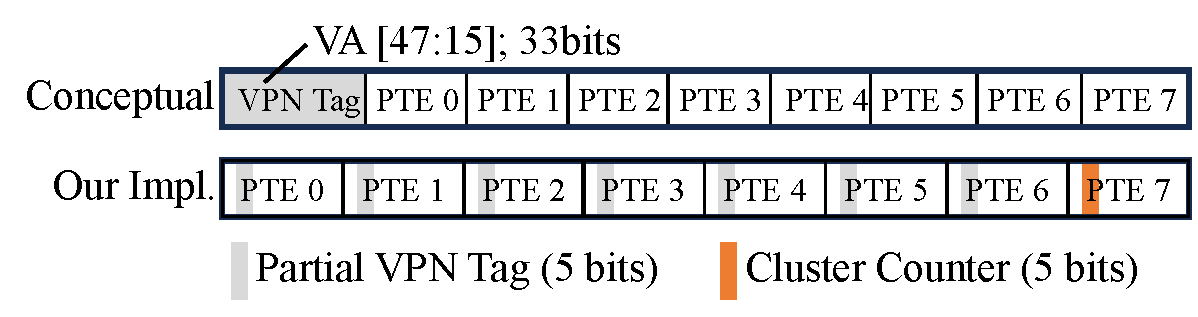
\includegraphics[width=0.6\textwidth]{figs/pte-cluster.pdf}
	\caption{{\bf Implementation of 64-byte PTE-ECPT entry clusters consists of eight 8-byte PTE entries.}
		Each entry contributes five bits for the VPN tag or a cluster count.
		}
%	\vspace{-5pt}
	\label{emt:fig:ecpt-impl:ecpt-cluster}
\end{figure}

When a table's occupancy exceeds a threshold (0.6 as in~\cite{skarlatos2020ecpt}),
	a background kernel thread resizes the table and migrates entries 
	from the old table to the new table gradually.

Except for the repurposed five bits for metadata,
	ECPT's translation entry by design follows 
	x86-64 PTE format.
We reuse the PTE encoding from the x86 radix MMU driver, enjoying 
	the benefit of EMT's object-oriented design.

Cuckoo Walk Tables (CWTs) are implemented in the ECPT MMU driver,
 	invisible to architecture-independent code.
We follow the ECPT design~\cite{skarlatos2020ecpt} to use a 5-bit section 
	header (a section is the address range translated by one 
	ECPT translation entry) and cluster 64 headers into a 64-byte cache line.
Each header is one byte and contributes three bits to encode the VPN tag and 
	count of valid section headers.

% \TODO{@Siyuan: write about how we implement the CWT entries.}
% By design, CWT uses 4-bit values to track the status of each 2M or 1G region, including if 4K pages are present in that region.
% For example, PMD-CWT uses a 4 bit section header to track mapping status of 16 MB memory region 
%	which is 8 2MB pages in a PMD-ECPT cluster.
%More specifically, one bit to indicate if it has 2M mappings, one to indicate if has 4K mappings,
%	the other two to indicate which way the 2M mappings are in.
% PUD-CWT uses 5 bits with one more to indicate if it has 1G mappings.
% In ECPT's design, 64 PMD/PUD-CWT section headers are clustered into a 64-bit cache line.
% We \TODO{TODO}.
% CWT updates are invoked by basic functions. % We update the PUD-CWT and PMD-CWT whenever a 4K or 2M cluster is inserted.

% \vspace{-1.5pt}
\para{Optimizations.} We implemented a series of optimizations through the customizable functions,
	driven by benchmarking and profiling (\S\ref{emt:ss:perf-ecpt}).
For example, we customize the iterator % \texttt{\small tentry\_iter\_next()} 
	% function %(Figure~\ref{emt:code:iternext}) 
	with architecture-specific optimizations
	to accelerate range operations.
The idea is to exploit locality within a translation entry cluster:
	the iterator finds the next entry by pointer arithmetic, instead of hashing-based lookups,
	when the entry is not the last one in its cluster. 
	%We show that this optimization leads to a major reduction of OS overhead (\S\ref{emt:ss:perf-ecpt}).
One common optimization pattern is to minimize the cost of range operations---the  
	default implementation (e.g., Figure~\ref{emt:code:iternext-gen}) often takes too many fine-grained hashing-based operations.
% \REVIEW{The iterator optimization reduces the cost of range operations, which are common routines in Linux --- 
% Without knowing the cluster organization, 
% the default implementation has to perform hash-based lookups repetitively.
% }
% \REVIEW{The iterator optimization reduces the cost of range operations, which are common routines in Linux --- 
% Without knowing the cluster organization, 
% the default implementation has to perform hash-based lookups repetitively.
% }
% We discussed the optimizations that avoid expensive range operations
%	in \S\ref{emt:sec:design:opt}.
% We also implement locks of different granularities for each entry cluster,
%	way, and tables other than the global ECPT lock.

% Please fix this time
% In fact, ECPT proposes axuliary data structure like CWT to track the mapping information.
% Unfortunately, since it was designed to reduce the number of parallel lookups,
%	it tracks mapping properties at a very coarse granularity,
%	which cannot directly help with \texttt{aspace\_partial\_built} implementation.

\begin{comment}
\para{Early page table setup}
Besides implementing the ECPT MMU driver and ECPT routines, we also need to prepare booting time page table for kernel.
It is buried under arch-specific code, but is a vital part of a workable kernel implementation.
\schai{Advise in this section}
In fact, if one is considering rebuilding kernel for a new translation architecture,
	I would recommend starting from the user page table setup for example in \S \ref{emt:sss:ecpt-init}.
Many of the routines are called in early stage of kernel booting,
	they are hard to understand and hard to debug.
For example, \texttt{\_\_startup\_64} prepares page table at the bootstrapping address space;
	an offset has to be added to get access to the real kernel address space.
Directly jumping to user page preparation will save a lot of time to understand what's benefit of user application with the new translation architecture.

Here we give a brief list of the most important steps and entry points for readers who wish to have a full Linux running on their own translation architecture:
\begin{itemize}
	\item Kernel text mapping \\
        \texttt{\_\_startup\_64} 
		% in \texttt{arch/x86/kernel/head64.c}
    \item Ioremap \& fixmap initialization \\
        \texttt{\_\_early\_set\_fixmap} 
		% in \texttt{arch/x86/mm/ioremap.c}
    \item Direct mapping for all physical memory \\
        \texttt{\_\_kernel\_physical\_mapping\_init} 
		% in \texttt{arch/x86/mm/init\_64.c}
    \item Data for sparse memory mgmt \\
        \texttt{vmemmap\_populate} 
		% in \texttt{arch/x86/mm/init\_64.c}
    \item CPU entry variables \\
        \texttt{cea\_set\_pte} 
	\item Change kernel memory attributes \\
		\texttt{set\_memory\_ro} ... 
		% in \texttt{arch/x86/mm/cpu\_entry\_area.c}
    \item Early PF handler \\
        \texttt{early\_make\_pgtable} 
		% in \texttt{arch/x86/kernel/head64.c}
\end{itemize}
\end{comment}

\subsection{Reflection on ECPT Design}
\label{emt:sec:reflection}

\noindent
We show that building OS components is essential to 
	understanding architecture designs.
	% , for 
	% both functionality and performance.
The efforts on developing and evaluating ECPT with EMT-Linux 
	reveals
% Developing and evaluating ECPT on EMT-Linux is a rewarding experience.
	OS challenges of  
	using a fast translation scheme, 
	which were unexpected (undocumented in the original hardware design).
% We address the challenge of managing the kernel page table (kECPT) 
%	(\S\ref{emt:ss:ecpt-kernelspace}) such as the paradox involved in modifying translations 
%	of the kECPT itself and of the kernel code that manages the kECPT.
% We reflect on the ECPT's hardware design and address the OS challenges,
%	some of which need new hardware support and OS cooperation.

\subsubsection{Managing Kernel Page Tables}
\label{emt:ss:ecpt-kernelspace}
%

\noindent
In modern OSes like Linux, the kernel address space is shared across processes~\cite{linux:mm}.
In tree-based translation, sharing is realized by having high-level
	page table entries pointing to the shared subtree of the kernel address space~\cite{linux:kpti}.
This design does not apply to hashing-based translation.
One option is to maintain one ECPT for
	each process containing both user- and kernel-space addresses. % \jzmark{If per-process, why we want to separate uECPT and kECPT? - The sole purpose to seperate is to share kECPT}
However, such a design is memory inefficient and leads to high overhead, e.g.,
	once a translation of a kernel-space address is updated, the OS must 
	update the corresponding entries in ECPTs of all processes.
% The original ECPT design only partitioned the page tables for different page sizes (4K, 2M, and 1G),
%	creating three set of page tables.
% However, modern operating systems 
%	such as Linux use a kernel address space that is shared across processes.
% Under ECPT design, when a page table is created for a process,
%	it needs to insert all translation entries regarding the kernel mappings into the process's page table,
%	which creates non neligible overhead.
% Even worse, when the kernel mapping is updated,
%	the kernel must update the page tables for all processes to reflect the changes in the kernel mapping.
	% this results in the kernel needing to update the page tables for each process,
	% so that they can correctly reflect updates to the kernel mapping.
% For simultaneous multithreaded systems, this design leads to additional synchronization overhead and
%	may potentially cause some processes to run on outdated mappings, which reduces system performance and stability.

Our ECPT MMU driver maintains a global kernel-space ECPT (kECPT) shared among processes 
	and an independent user-space ECPT (uECPT) for every process.
The kECPT has the same page size and way configuration as each uECPT.
The kECPT and uECPTs are managed independently.
When KPTI (kernel page table isolation)~\cite{linux:kpti} is enabled, 
	two independent global kECPTs are managed
% We find such a design is elegant and supports features like 
	(a complete kECPT and a minimal kECPT).
This design requires ECPT MMUs to expose another nine control registers that point 
	to kECPT(s).\footnote{
\schai{
	The cost of additional architectural registers is negligible; they add to less than 0.01\% of the die area.
	The area overhead was measured with the same methodology as in ~\cite{skarlatos2020ecpt,jovan2022nestedecpt} using CACTI~\cite{cacti} with 22nm technology. 
	The new design also distinguishes whether the target address belongs to the upper or lower half of the address space and directs the lookups to uECPT or kECPT. 
	CWC is shared and has no additional cost.}} 
% Whether to use the same sets of hash functions for kECPT and uECPT is an architectural design choice; independent sets add cost.
	
% 	\footnote{
% \schai{
% 	The cost of additional architectural registers is negligible; they add to less than 0.01% of the die area 
% 	(measured with the same methodology as in ~\cite{skarlatos2020ecpt} using CACTI with 22nm; we also scale it to 7nm based on [A]). 
% 	The new design also distinguishes whether the target address belongs to the upper or lower half of the address space and directs the lookups to uECPT or kECPT. 
% 	CWC is shared and has no additional cost. Whether to use the same sets of hash functions for kECPT and uECPT is an architectural design choice; independent sets add cost.}
% 	}
% \schai{The cost of additional architectural registers is very small. Whether to use the same sets of hash functions for kECPT and uECPT is an architectural design choice; independent sets add cost.}

% The cost of additional architectural registers is very small; they add to less than 0.01\% of the die area (measured with the same methodology as in [91] using CACTI with 22nm
% \jzx{and a register to mark the kernel-user mapping boundary}{} \TODO{@Jiyuan: why we need this?}. \jzmark{The marking register is not required (and it does not present in our implementation) - x86/ECPT PTE has a Supervisor/User bit to do that marking already}

% To tackle this problem, we maintain two set of page tables one for kernel space the other for user space.
% From the OS side, two set of page tables are maintained independently:
%	kernel mapping udpates go to the kernel page table, and user mapping updates go to the user page table.
% When a process is created, we just allocate its user page table with \texttt{init\_addr\_space} interface;
%	the kernel page table is untouched.
% When we context switch to a process, we update user page table's register with process's user page table
%	and kernel page table's register with kernel page table.
% We avoid incurring overhead of inserting kernel mapping into user page table.
% When a kernel mapping is updated, we only need to update the kernel page table.
% Whenever a process switched in, it will get the latest kernel mapping
%	without updating all processes' page tables.
% Such modification allows all kernel threads to work on an up-to-date mapping and avoids the overhead of updating multiple page tables.
% However, this modification requires the hardware to expose additional page table registers.
% From the HW side, we add 6 registers for kernel page tables (3 for 2M and 3 for 4K following ECPT's design)
%	and one register to distinguishe the kernel-user mapping boundary
%	so that hardware only reads from kernel page table when it can tell it's a kernel mapping.

% For future hardware design, people may need to think about how to efficiently share kernel mappings across processes
%	since this is a common practice in modern operating systems to support advanced features page table isolation.
% Radix relies on kernel to maintain a subtree of page tables for kernel mappings.
% ECPT can be enhanced with our idea of maintaining two set of page tables.

\para{Self-Reference Paradox.}
\label{emt:ss:ecpt-self-reference}
Managing kECPTs is more challenging than uECPTs.
Different from uECPTs that are mandated by the kernel, 
	the kECPT manages the kernel's own code and data---translations 
	for kECPT management code and kECPT itself
	are stored in kECPT.
This creates a challenge for ECPT which needs to move translation entries 
	across ways for resolving hash collisions---in the
	moving window, if the entries map the kECPT itself 
		or the kernel code for moving entries are missing,
		the kernel crashes due to missing translation of the kECPT or code,
		as shown in Figure~\ref{emt:fig:ecpt-impl:paradox}.
Frequent triggers are kernel's huge page promotion/demotion
	which remove entries and insert new entries in different tables. 

We term the issue {\it self-reference paradox}. The root cause is a lack of hardware support 
	for atomic updates on multiple memory locations.
Radix-tree page tables do not face this paradox, because 
	they do not move entries and the huge-page promotion/demotion is done by updating one PUD/PMD entry.
In general, the self-reference paradox can happen in kernel page tables
	that need to move entries (many advanced index schemes need to move entries~\cite{Bender2023,zuo2018}). %, e.g.,~\cite{Bender2023}.
Note that other kernel structures like
forwarding table~\cite{zhou2013cuckooswitch} do not face this paradox if they do 
	not map kernel code/data.

% The root cause of the problem here is that ECPT's page table design requires
% updating multiple location in the page table in kicking and changing between 2M and 4K mappings, 
% but no modern architecture can support atomic updates across mulitple positions.
% On the contrary, radix avoids this issue because of its tree based nature.
% It never needs to resolve hash collision, and changing between 2M and 4K mappings
% only involves single L2 entry update.

%	Say kernel text and page table's are mapped by 2M entries in ECPT.
%	When kernel want to split a 2M entry into 512 4K entries, 
%		it needs to remove the 2M entry and insert 4K entries.
%	If removal goes before insertion, there will be a transient stage in between kernel misses mapping.


% Just as every user process, kernel runs in its virtual address space.
% Differently, it manages its own page table while all of its code relying on the self-managed page table to run.
% Different from a user process, kernel manages its own page table
%	which maps all kernel text and data.
% Kernel works in within virtual address space;
% 	it relies on kernel page table to map kernel text and data.
% More importantly, mappings for kernel's text for page table management
%	and the in-memory page table itself are stored in the page table.
% Since the operating system kernel works on the kernel virtual address space,
	% it relies on 
	% it needs to use virtual addresses to access and manage page tables and physical memory mappings.

% Hence, the page table must correctly maintain the PTEs that map the page table itself and associated routines into the kernel space;
%	otherwise, the kernel will lose access to the page table or corrupt in the middle of running.

% \jztodo{one example is enough - correctness is an instant kill so don't need to hits - focus on the solution more}
% However, our tests found that this requirement conflicts with
%	ECPT's kicking routine to resolve hash collision.
% During kicking, kernel migrates PTEs from old page table to new page table,
% However, our tests found that this requirement conflicts with ECPT's rehash mechanism.
% In the process of kicking a PTE from a old ECPT way to new way,
%	kernel removes in old way and inserts it into the new way.
% In the process of migrating the PTEs used to map the page table itself,
	% the kernel needs to remove the PTEs from the old table and insert them into the new table.
% Yet, if the PTE maps the page table itself or exactly kicking routine's kernel text,
%	during the transient stage between removal and insertion,
%	kernel loses access to the page table or corrupt itself due to missing text mapping.

\begin{figure}[H]
	\centering
	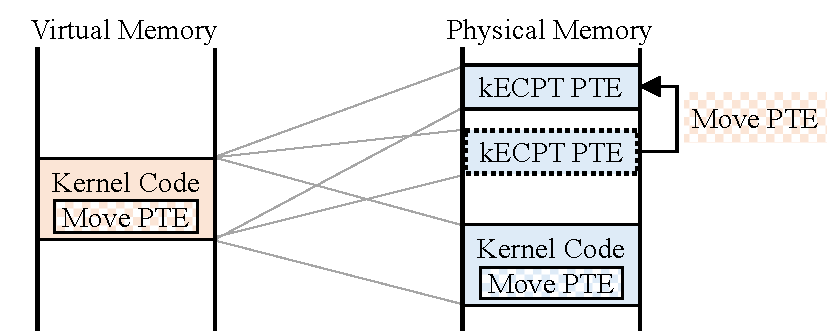
\includegraphics[width=0.52\textwidth]{figs/paradox.pdf}
	\caption{{\bf An example of self-reference paradox caused by the need of 
		moving kECPT entries that are needed to find kernel code
		for moving kECPT entries (\S\ref{emt:ss:ecpt-self-reference}).}}
%	\vspace{-7.5pt}
	\label{emt:fig:ecpt-impl:paradox}
\end{figure}

We address the paradox via a series of software-hardware endeavors.
First, we always copy the entry to the new location {\it before} removing it at the old location,
	which may cause duplicated entries but no missing entries.
We instruct the MMU to handle duplicate entries that have the same virtual-to-physical address mapping 
	and the same protection bits; the deduplication policy also works
	for huge-page promotion/demotion as it does not change the mapping or protection.
We avoid location-changing read-update-write operations in OS code % to have different sources and destinations
	so that duplicated entries always have the same mapping and protection. %, to avoid ambiguity in mapping information.
For ECPT, any operation that may change the content of an entry
	can only be done after the entry is locked.

%	However, such an attempt will cause multiple PTEs to map the same address space simultaneously,
%		which is contrary to fundamentals of virtual address design where one VA should mapped to a single PA.
% In such way, it requires additional hardware logic to arbitrate which PTE to use, reducing the stability of the system.
% We patch the hardware to allow multiple PTEs to map the same address space,
%	if they points to the same physical address and have the same permission. 

% Future hardware design should consider the neccessity of multi-location update in page table design.
% If that is a must,
%	it needs to specify the order of update desired and provide a clear defined way to handle transient stage of duplicated mappings.

\para{Atomic kECPT Switching.}
% \paragraph{Inconsis kECPT during switch}
\label{emt:sec:split_kecpt}
Another form of self-reference paradox manifests
	via KPTI~\cite{linux:kpti}---when switching 
	% \schaix{from the kernel space to the user space}
	\schai{between the kernel space and the user space},
	the OS needs to switch 
	% \schaix{from a full kECPT to a minimal kECPT} 
	\schai{between a full kECPT and a minimal kECPT}. 
One potential implementation is to use multiple \texttt{\small mov} instructions to redirect control registers 
		from the old kECPT ways to the new ways.
However, this may lead to an inconsistent ECPT state during the switch window, 
	where some registers point to new ways and the others point to old ways.
This leads to issues 
	when the translations of currently executing kernel code 
	are stored in different ways across the new and old kECPTs.
\schai{Note that simply keeping context switch code covered by both kECPT is not enough
since the instructions can reside in different ways of the old and new tables.
Instructions might not be successfully fetched when kECPT state is inconsistent.
}

Solving this problem needs a mechanism for atomic switching from all 
	old kECPT ways to the new kECPT ways.
Such an atomic switching mechanism can be realized with hardware support. 
% To solve this problem, \jzxc{we would need a single serializing instruction for the switch
%	so the hardware must complete all updates for switching
%	before the next instruction can execute.}{all the way switches should happen simultaneously to maintain address space consistency,
%		ideally enabled by hardware support, e.g. a special instruction.}
%			{serializing does not guarantee simultaneity, don't abuse term}
% \jztodo{@siyuan: why ECPT has CR3? what's the purpose?}
Our solution is to add additional sets of kECPT control registers 
	and the hardware switches between the two sets of control registers,
	in a similar vein as the \texttt{VMLAUNCH} and \texttt{VMRESUME} instructions of x86
	on updating multiple registers together.
The switch is a serializing instruction to ensure 
% The kernel switches to new kECPT by updating CR3, a serializing instruction in x86 ISA;
that all instructions after it will use the new kECPT.

% \schai{This will cause trouble since the later \texttt{\small mov} instructions may 
%	need kernel text fetch which requires access the old kECPT.
% We need a switch with a single serializing instruction;
%	in other words, the hardware must 

% However, without atomicity, the system will be in an inconsistent state 
% 	during the switch,
% 	where some registers pointing to the new tables
% 	and the others pointing to the old tables.

% \schai{
% We solved this problem with collective force from hardware and kernel.
% We added two sets of kECPT control registers 
	
% }

% \begin{figure}[t]
% 	\centering
% 	\begin{subfigure}[b]{0.5\textwidth}
% 		\centering
% 		
\includegraphics[width=\textwidth]{data/radix_lebench_legend.pdf}
% 		% 
\includegraphics[width=\textwidth]{data/radix_lebench_single_legend.pdf}
% 	\end{subfigure}%
	
% 	\vskip\baselineskip
% 	\vspace{-14pt}
% 	\makebox[1\textwidth][c]{%
% 		\begin{subfigure}[t]{0.75\textwidth}
% 			\centering
% 			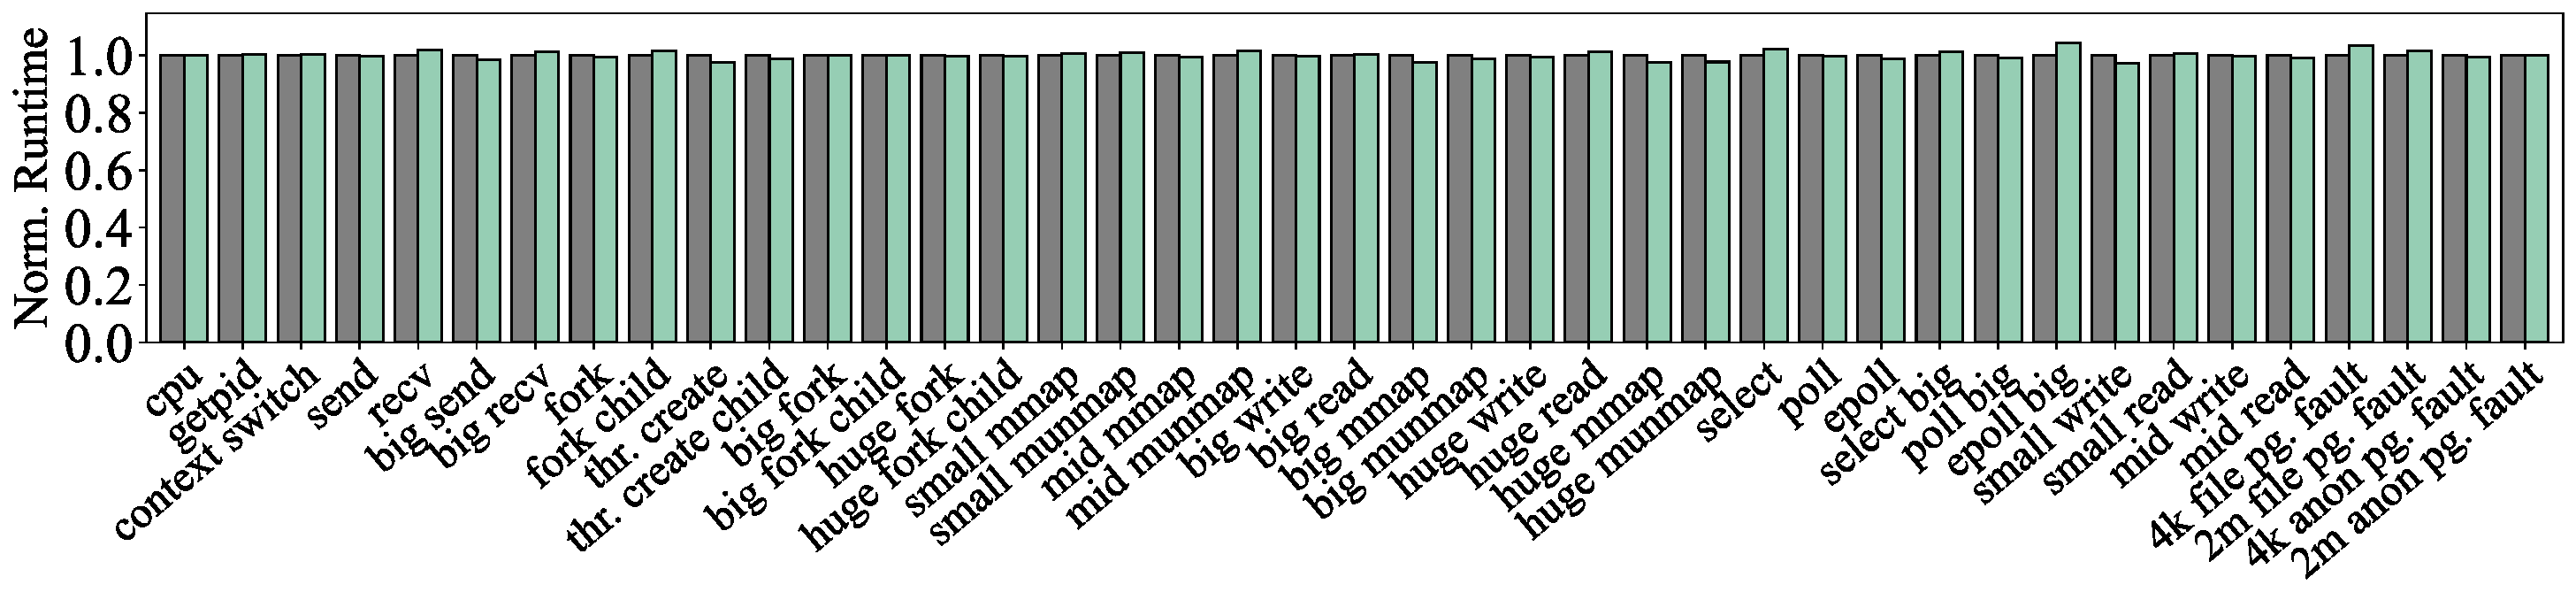
\includegraphics[width=\textwidth]{data/radix_lebench.pdf}
% 			% \includegraphics[width=\textwidth]{data/radix_lebench_double.pdf}
% 			\captionsetup{justification=centering}
% 			\vspace{-24pt}
% 			\caption{Micro benchmark}
% 			\label{emt:fig:eval:microbenchmark}
% 		\end{subfigure}
% 		\hfill
% 	\raisebox{16.5pt} {
% 		\begin{subfigure}[t]{0.25\textwidth}
% 			\centering
% 			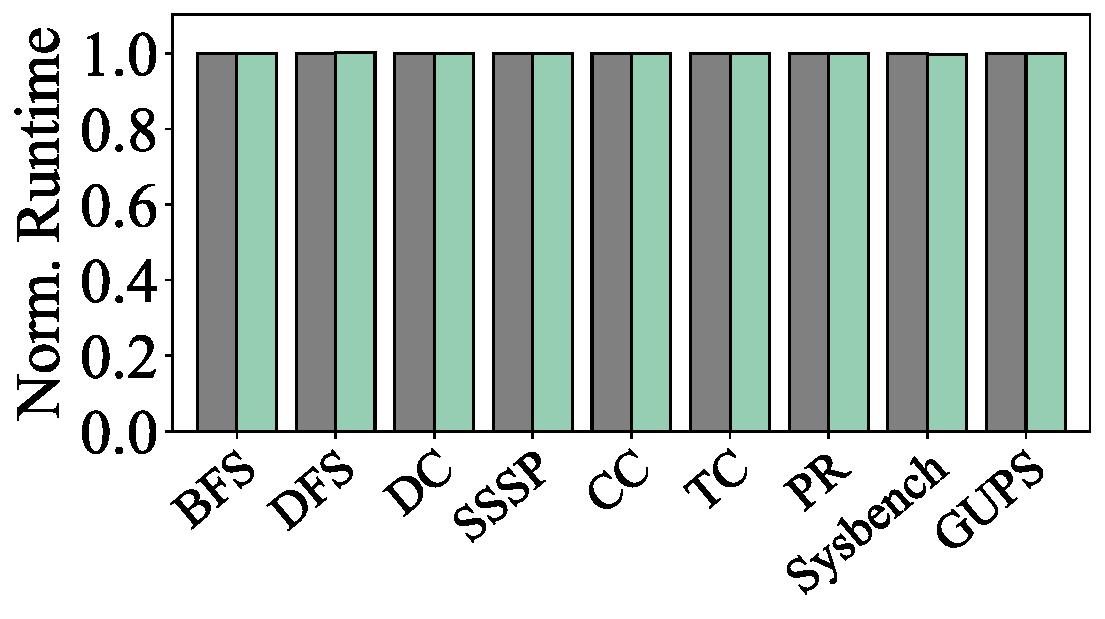
\includegraphics[width=\textwidth]{data/radix.pdf}
% 			% 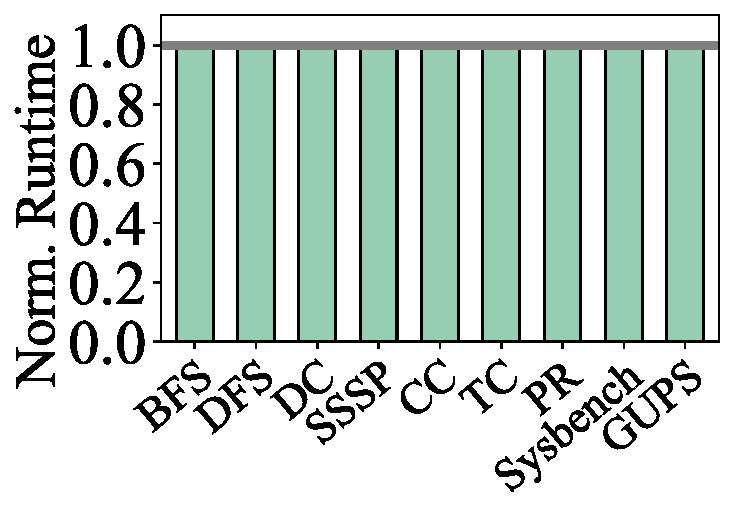
\includegraphics[width=\textwidth]{data/radix_single.pdf}
% 			\captionsetup{justification=centering}
% 			\vspace{-12pt}
% 			\caption{Macro benchmark}
% 			\label{emt:fig:eval:macrobenchmark}
% 		\end{subfigure}
% 	}
% 	}
% %	\vspace{-12pt}
% 	\caption{\bf Performance overhead of EMT-Linux over vanilla Linux (measured by the micro and macro benchmarks).}
% 	\label{emt:fig:eval:eval-stack-lebench}
% %	\vspace{-5pt}
% \end{figure}

\begin{figure}[H]
	\centering
	\begin{subfigure}[b]{0.5\textwidth}
		\centering
		
\includegraphics[width=\textwidth]{data/radix_lebench_legend.pdf}
	\end{subfigure}%
	
	\vskip\baselineskip
	\makebox[1\textwidth][c]{%
		\begin{subfigure}[t]{0.75\textwidth}
			\centering
			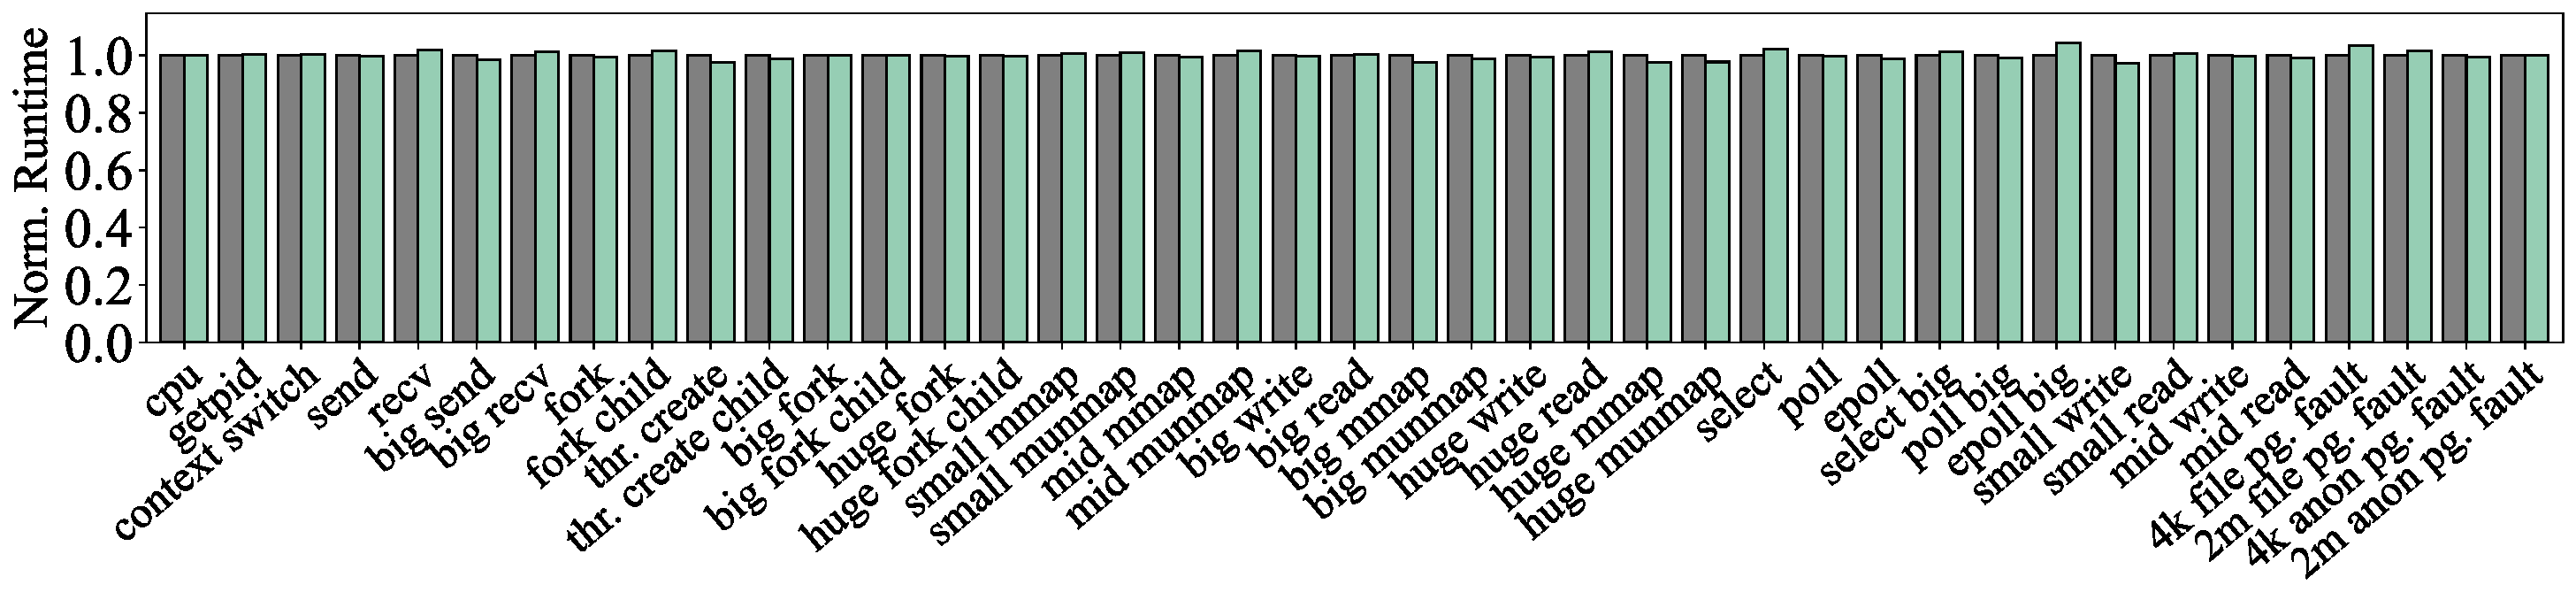
\includegraphics[width=\textwidth]{data/radix_lebench.pdf}
			\captionsetup{justification=centering}
			\caption{Micro benchmark}
			\label{emt:fig:eval:microbenchmark}
		\end{subfigure}
		\hfill
	\raisebox{16pt} {
		\begin{subfigure}[t]{0.25\textwidth}
			\centering
			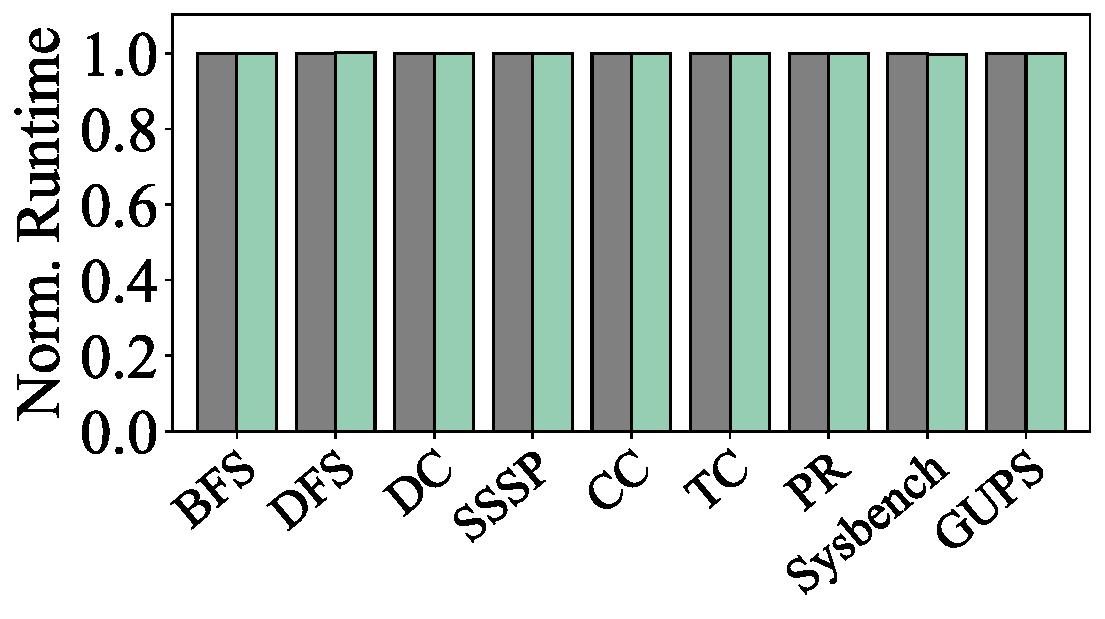
\includegraphics[width=\textwidth]{data/radix.pdf}
			\captionsetup{justification=centering}
			\caption{Macro benchmark}
			\label{emt:fig:eval:macrobenchmark}
		\end{subfigure}
	}
	}
	\caption{\bf Performance overhead of EMT-Linux over vanilla Linux (measured by the micro and macro benchmarks).}
	\label{emt:fig:eval:eval-stack-lebench}
\end{figure}

% We add hardware support for atomic kECPT switching.
% 	considering current x86 processors already explicitly serialize change to the CR3 register.
% The MMU provides two sets of kECPT control registers and
% 	\schai{we repurpose a bit reserved bit in cr3 to switch} between them 
% 	with no memory access or transient state in between.
% Update to cr3 is a serializing instruction in x86, 
% 	our design ensures that the hardware completes all updates 
% 	before the next instruction can execute

%	the switching can be preloaded into the inactive set.
%After the loading is done, the hardware can atomically toggle to the new set of registers and render the previous ones inactive,
%	avoiding any memory accesses and transient state in between.

% \schai{
% One solution is to add 9 more registers as scrachpad 
%	in addition to original 9 registers to store the new kECPT's way information.
% We can repurpose a bit in cr3 to indicate which set of registers to use. 
% Once the scrachpad registers are all updated,
%	we can flip the bit in cr3 to make the new registers effective.
% The other solution is to update cr3 register pointing to an array containing the new kECPT's way information.
% Once the cr3 is updated, the hardware will automatically update the control registers associated with new kECPT.
%
% In both solution, no kernel instruction will be executed nor any memory access will be made 
%	until the entire switch is complete.
% The first solution requires little hardware logic change, and may be preferred in reality.
% }


% (tianyin) atomicity is referring to the operation; serializing instruction is the implementation,
% but I don't know how serializing instruction helps *multiple* CR registers still :()
% \schaic{I think atomicity is a stronger assumption than we need. 
% All we need is a single serializing instruction that finishes the change. 
% aka, proecessor complete all updates to the instruction, before next instruction can execute.
% mov cr3 is a classic serializing instruction.}
\subsubsection{Implications on OS Performance}
\label{emt:sec:ecpt:os:perf}

\noindent
% We show that ECPT has profound performance implications on OS memory management,
%	especially in terms of 
%	its ability to manage sparse address space
%	and multicore scalability.
{\bf Managing Sparse Address Space.}
\label{emt:sec:reflection:sparse}
% Despite optimizations that utilize spatial locality of clustered entries,
%	range operations in ECPT are still much more expensive than radix page tables.
% However, managing large address ranges is a common memory management operation pattern.
A fundamental efficiency property of tree-based page tables is the 
	ability to manage sparse address space, which is critical for 
	OS memory management which commonly needs to scan large, but sparse address ranges.
In tree page tables, a high-level entry
	can encode properties of a large address range, e.g.,
	% (e.g., whether it has any allocated pages and their sizes).
	a nonexistent PMD entry indicates no valid page allocated in the corresponding 2MB range.
%	hence, the OS only needs to check one entry instead of all the possible PTE entries in the space.
Hashed page tables have no such hierarchical relationship between entries;
	hence, the OS may go through all the possible entries in the large, sparse address range.

One optimization is to enable a similar property in ECPT by designing 
	special entries that are not for translation, but for encoding states. 
The OS checks the entry to learn the states of the corresponding address range, e.g.,
	the OS can query such an entry to check if the corresponding 2MB address range has 
	any allocated page, instead of checking all possible PTE entries.
The design would need to cooperate with the MMU. % to avoid confusion.
% no, it does not add anything
% \jztodo{Shall we mention this does not require hardware change? - it's purely for the OS's need}

\begin{comment}
\jz{Such special entries have additional benefits in maintaining coherency between ECPT and its translation caches (CWC/CWT).
ECPT CWC/CWT uses a single bit to encode whether or not any 4KB page presents in a 2MB region,
	hence helping decide whether accesses to 4KB ways are necessary.
However, while the set of such a bit is trivial (set on the first 4KB page allocation),
	clearing it requires a proper counting mechanism.
The special entries can serve this purpose and help count 4KB pages in a region.
Once the counter drops to zero, the CWC/CWT bits can be promptly and safely cleared.
}
\end{comment}

% ECPT uses software-maintained Cuckoo Walk Tables and its hardware-cached subset, the Cuckoo Walk Caches,
%	to reduce the number of parallel lookups.
% By design, CWT uses 4-bit values to track the status of each 2M or 1G region, including if 4K pages are present in that region.
% For example, PMD-CWT uses a 4 bit section header to track mapping status of 16 MB memory region 
%	which is 8 2MB pages in a PMD-ECPT cluster.
% More specifically, one bit to indicate if it has 2M mappings, one to indicate if has 4K mappings,
%	the other two to indicate which way the 2M mappings are in.
% PUD-CWT uses 5 bits with one more to indicate if it has 1G mappings.
% Kernel will set 4K bit whenever a 4K mapping is inserted into the region,
%	but it doesn't know when to clear it since it doesn't know 
%	when the last 4K mapping is removed in the 16MB region.

% However, recall that each 2M region has 512 4K pages, CWT by design cannot track the count of 4K pages in a region.
% However, recall that each 2M region has 512 4K pages, CWT by design cannot track the count of 4K pages in a region.

% \paragraph{High Memory Usage}

% \begin{center}
% 	\jztodo{Table: Fill in the number}
% 	\begin{tabular}{||c c c c||} 
% 	 \hline
% 	 Benchmark & Radix & ECPT claimed & ECPT \\ [0.5ex] 
% 	 \hline\hline
% 	 1 & 6 & 87837 & 787 \\ 
% 	 \hline
% 	 2 & 7 & 78 & 5415 \\
% 	 \hline
% 	 3 & 545 & 778 & 7507 \\
% 	 \hline
% 	 4 & 545 & 18744 & 7560 \\
% 	 \hline
% 	 5 & 88 & 788 & 6344 \\ [1ex] 
% 	 \hline
% 	\end{tabular}
% 	\end{center}
% % The scripts they use always resize to the optimal space arrangement (or even lower than optimal)
% % Hence, despite their script is lost, the following two points can still stand.

% In practice, ECPT exhibits much higher memory usage than what is documented in the original paper even with all optimizations applied (\S\ref{emt:sec:ecpt-opti}), as shown in Table \ref{}\JZtodo.
% Such difference is potentially due to two factors:
% %
% First, the original paper assumes that ECPT always picks optimal resize decisions.
% However, in real runs, ECPT inserts PTEs into random ways, and thus, the optimal resize decision is not always made.
% % However, in real runs, the information used for such decision-making is not always available, and thus, the memory space overhead will increase.
% %
% \JZtodo \schaic{@Jiyuan, can you speicify this, I don't find how they explain x4 resizing in paper}.
% Second, a portion of hash collisions cannot be resolved after a single resizing/rehashing.
% This results in a chained resizing attempt, quadrupling the size of the page tables.
% However, this additional space waste due to hash collisions was not accounted for.

% \jztodo{@tianyin: probably we need to change our tone on memory usage?}

% % \jztodo{@siyuan: a table comparing vanilla x86, paper ECPT, and actual ECPT memory usage}


% There are multiple ways to reduce the memory usage for a hash page table design
% 	\ref*{} 
% % Jovan paper.
% Instead, we propose a software technique to reduce memory usage from a system perspective.
% In the original ECPT design, all ECPT size tables were eagerly created.
% However, we observe that in real systems, not all applications use huge pages.
% For these applications, their 2M and 1G size tables are always idle, wasting memory space and continuity.
% To optimize, our ECPT MMU driver by default points all 2M and 1G size tables to a globally shared dummy table.
% It only creates 2M and 1G tables when a process allocates huge pages for the first time.

\begin{comment}
\paragraph{PTE bits and swap space}
It's common for a hash page table design to repurpose bits 
	in PTEs to store auxilary information for the page table.
For example, ECPT repurposes 5 bits from each PTE to store the virtual page number for that cluster.
While the pte itself is only used as a translation entry,
	the interface can well hide the its complexity 
	by doing inserting and removing operations respecting bits repurposing.
However, in Linux, it will mark a pte as not present but still stored in page table,
	when it is swapped out to disk or marked as migration entries.
The marking is done by converting the pte entries to swap entries,
	when the page is brought back in memory, the swap entries are converted back to pte.
% treated a pte as swap entry when it is swapped out to disk,
% 	or marked as migration entries.
% A swap entry is converted from pte based on values in pte.
Both conversion process directly operate on the bits in pte.
Repuproposing the bits in pte without considering its conversion to swap entry
	can lead to a swap entries with wrong indexing
	or the ptes converted back points to wrong memory location.

With our interface, the system can be exhaustively tested to ensure 
	that swap entries are correctly formatted and converted back to pte.
Implementing the pte's \texttt{read\_entry\_attr} and \texttt{write\_entry\_attr} interface
	can help to ensure the correctness of the swap entries.
During our implementation, we find that since the we have to preserve the bits in pte,
	they can not be reused in swap entries to index the swap space,
	which brings the side effect by cutting down available swap space the system can have
	by a factor of 2\^5 (the remaining size is still 2\^54 pages).
This appears acceptable right now, but may be a problem if designers want to repurpose more bits in pte
	or wants to have a larger swap space.
\end{comment}

% \subsubsection{Implemented and Potential Optimizations}
% \label{emt:sec:ecpt-opti}

% % \paragraph{PTE Clustering}

% % In the original ECPT design, as each PTE is independently hashed, hashes need to be computed for each PTE, which leads to high software overhead.
% % To reduce this overhead, we modify the ECPT design to provide a hash slot for every 8 consecutive PTEs.
% % The new design places adjacent PTEs consecutively in hash slots.
% % Our evaluation in \S\ref{}\JZtodo shows that this optimization drastically reduces the number of hash computations necessary
% % 	when performing address range operations, leading to a \jztodo{@siyuan: 100}\% reduction in overall software overhead
% % 		with a hash slot utilization of \jztodo{@siyuan: 100}\%. % I put this utilization thing here to defend against suspicion on "space waste"

% \paragraph{On-Demand Size Table Creation}

% In the original ECPT design, all ECPT size tables were eagerly created.
% However, we observe that in real systems, not all applications use huge pages.
% For these applications, their 2M and 1G size tables are always idle, wasting memory space and continuity.
% To optimize, our ECPT MMU driver by default points all 2M and 1G size tables to a globally shared dummy table.
% It only creates 2M and 1G tables when a process allocates huge pages for the first time.

% This is weird to write and I think could contradict to an arch-generic interface.
% \paragraph{Tracking Non-leaf PTE}

\para{Multicore Scalability.}
\label{emt:sec:multithreading}
% We have not extensively evaluated the multi-core scalability 
%	of ECPT on EMT-Linux where multiple kernel threads 
%	concurrently change the same table or way in ECPT.
We find it nontrivial to implement efficient 
	locking primitives similar to 
	Linux's split page table lock~\cite{linux:sptl} in ECPT,
	because % hashes page table entries of adjacent addresses into different locations
	the location of an ECPT entry can be moved due to insertion or rehashing.
The movement of entries makes it prone to deadlocks, e.g.,	
	one thread $t$ holding a lock $l$ and inserting a new entry,
	thus consequently requires moving an existing entry $e$ (see~\cite{pagh2004cuckoo}) which 
	is locked by another thread that waiting on $l$.
% Empirically, we find that such deadlocks rarely occur.
% \schaix{Empirically, we find that such deadlocks rarely occur.}
One solution is to let $t$ release all its acquired locks 
	and retry later when deadlock.
The complexity lies in recording and rewinding states changed by $t$.
We are exploring an alternative design that introduces a separate lock table to provide the OS 
	with the flexibility of implementing lock primitives, which has the semantic of locking both an address range 
		and the related entries.
\schai{Our implementation of the ECPT MMU driver has no correctness issue, as we use a coarse-grained lock.}
%	decoupling lock implemenations from the translation architecture. % , which is often optimized for hardware rather than software.
% The OS may use a tree of linked lists for split page table locks~\cite{linux:sptl}.

% \jz{Before each update operation, the MMU driver can check the external tree to confirm whether
%	the pending operation is blocked by some locks or not.
% In this way, one can rule out the chance that an operation accidentally interferes with the critical section for others.}
%	and support different levels of locks.
% During each lock-dependent operation,
%	the OS and MMU driver routines can check the lock status table to observe the locked status,
%	and take and hold address range locks exclusively from the table.
% For ECPT, one can repurpose spare bits in CWT entries to implement spinlocks,
%	as CWT entries cover larger memory regions than translation entries \jz{and are immune to the hashing side effect}. 
% \JZc{I found seperate lock table does not help the deadlock, only locking the entire kicking chain do}

%		\jz{of unrelated entries -- which renders page table operations having a larger scope of impact than what is explicitly changing}.
% 2) the location of a page table entry may change even when the VA-PA mapping is not changing, due to kicking or rehashing,
% and 3) unlike x86, ECPT does not reserve blank slots for memory holes, hence memory holes cannot be locked without inserting dummy entries first.
% Hence, to lock an address range, % to external changes,
%	a thread must lock every entry,
%	which in itself is expensive and may wait for \jzx{unrelated locks of other memory regions}{all kicking and rehashing operations to settle to avoid deadlock}.
% \schaic{
% Actually, I think this may not happen, for a range lock. Thread A should wait for B,
% since range lock is a acquired at once. If B holding the lock for E4 which is already in table,
% 	then A shouldn't be able to hold the lock and wait. It should finish operation on E1-E3 range,
% 	then try to acquire lock for E4's range.

% % Even if the scenario may happen, in practice, the probiblity is extremely extremely low.
% % Let's say all ECPT ways have size of T, then for P( h(E') \% T == h(E1) \% T) = 1/T.
% % If that happens for all E2, E2, E3, then the probility is (1/T)\^3.
% % Given T >= 16K. The probablity goes is about 2.27e-13.
% % Even if thread A is holding lock for n entries, n < 2M/4K/8 = 64 entries if we have 2M has lock granularity,
% % and n < 16M/4K/8 = 512 entries if we have 16M as lock granularity.
% % Then, the probability in this case becomes (n/T)^3, which is still very very low.
% % In that case, we can tolerate the insertion failure by retrying.
% }

% \jzmark{Imagine two threads where: (1) Thread A locked PTE E1-E3 and waiting on lock E4 to proceed;
%	(2) Thread B is inserting a new PTE E' while holding the lock for E4.
% A tricky thing that can happen is: (1) E' can only go to E1-E3 as collision is purely random (so there is always a chance),
%	hence B is waiting on A;
% (2) A is also waiting on B (via E4 lock);
% (3) rehash is not possible as external users (Thread A/B) are holding locks.
% This constitutes a deadlock scenario.}



\begin{comment}
% When the Linux kernel updates page tables, it needs to take the page table lock.
% Locking the entire page table is not scalable in a multi-threading environment.
Hence, Linux takes a lock-the-sub-table approach: 
	it associates each page table page with a memory page lock that serves as a sub-table lock.
The lock appears to lock the page table data page 
	but also semantically locks the virtual address range associated with the page table page.
However, this locking practice assumes that page tables have a hierarchical architecture (which is not the case for hash and deleveled page tables)
	and that page table pages correspond to fixed address space ranges on a page-by-page basis (which is not the case for hash and adaptive page tables).
Such an assumption comes from the implied spatial feature that all page table entries associated 
	with the virtual address range are stored in the same page table page and the relation is immutable.
For page table designs that don't have such organization,
	locking a page table page will of course not lock the correct virtual address range.
\end{comment}

\begin{comment}
In the end, for the locking use case scenario, the proposed abstraction must simultaneously satisfy at least four constraints:
	1) support multi-granularity address range locking capabilities, 
	2) awareness of the locking status of address range subsets and supersets,
	3) do not implicitly require the page table to be hierarchical,
	4) respect the run-time variability of the page table structure itself.
\end{comment}
